%% Преамбула TeX-файла

% 1. Стиль и язык
\documentclass[liberation]{G7-32}

% Остальные стандартные настройки убраны в preamble.inc.tex.
\sloppy

% Настройки стиля ГОСТ 7-32
% Для начала определяем, хотим мы или нет, чтобы рисунки и таблицы нумеровались в пределах раздела, или нам нужна сквозная нумерация.
\EqInChapter % формулы будут нумероваться в пределах раздела
\TableInChapter % таблицы будут нумероваться в пределах раздела
\PicInChapter % рисунки будут нумероваться в пределах раздела

% Добавляем гипертекстовое оглавление в PDF
\usepackage[
bookmarks=true, colorlinks=true, unicode=true,
urlcolor=black,linkcolor=black, anchorcolor=black,
citecolor=black, menucolor=black, filecolor=black,
]{hyperref}

\AfterHyperrefFix

\usepackage{microtype}% полезный пакет для микротипографии, увы под xelatex мало чего умеет, но под pdflatex хорошо улучшает читаемость

% Тире могут быть невидимы в Adobe Reader
\ifInvisibleDashes
\MakeDashesBold
\fi

\usepackage{graphicx}   % Пакет для включения рисунков

% С такими оно полями оно работает по-умолчанию:
% \RequirePackage[left=20mm,right=10mm,top=20mm,bottom=20mm,headsep=0pt,includefoot]{geometry}
% Если вас тошнит от поля в 10мм --- увеличивайте до 20-ти, ну и про переплёт не забывайте
\geometry{ignorefoot}% считать от нижней границы текста


% Пакет Tikz
\usepackage{tikz}
\usetikzlibrary{arrows,positioning,shadows}

% Произвольная нумерация списков.
\usepackage{enumerate}

% ячейки в несколько строчек
\usepackage{multirow}

% itemize внутри tabular и выравнивание таблиц
\usepackage{paralist,array,tabularx,tabulary}
\newcolumntype{C}{>{\centering\arraybackslash}X}

%\setlength{\parskip}{1ex plus0.5ex minus0.5ex} % разрыв между абзацами
\setlength{\parskip}{1ex} % разрыв между абзацами
\usepackage{blindtext}

% Центрирование подписей к плавающим окружениям
%\usepackage[justification=centering]{caption}


% Настройки листингов.
\ifPDFTeX
% 8 Листинги

\usepackage{listings}

% Значения по умолчанию
\lstset{
  basicstyle= \footnotesize,
  breakatwhitespace=true,% разрыв строк только на whitespacce
  breaklines=true,       % переносить длинные строки
%   captionpos=b,          % подписи снизу -- вроде не надо
  inputencoding=koi8-r,
  numbers=left,          % нумерация слева
  numberstyle=\footnotesize,
  showspaces=false,      % показывать пробелы подчеркиваниями -- идиотизм 70-х годов
  showstringspaces=false,
  showtabs=false,        % и табы тоже
  stepnumber=1,
  tabsize=4,              % кому нужны табы по 8 символов?
  frame=single
}

% Стиль для псевдокода: строчки обычно короткие, поэтому размер шрифта побольше
\lstdefinestyle{pseudocode}{
  basicstyle=\small,
  keywordstyle=\color{black}\bfseries\underbar,
  language=Pseudocode,
  numberstyle=\footnotesize,
  commentstyle=\footnotesize\it
}

% Стиль для обычного кода: маленький шрифт
\lstdefinestyle{realcode}{
  basicstyle=\scriptsize,
  numberstyle=\footnotesize
}

% Стиль для коротких кусков обычного кода: средний шрифт
\lstdefinestyle{simplecode}{
  basicstyle=\footnotesize,
  numberstyle=\footnotesize
}

% Стиль для BNF
\lstdefinestyle{grammar}{
  basicstyle=\footnotesize,
  numberstyle=\footnotesize,
  stringstyle=\bfseries\ttfamily,
  language=BNF
}

% Определим свой язык для написания псевдокодов на основе Python
\lstdefinelanguage[]{Pseudocode}[]{Python}{
  morekeywords={each,empty,wait,do},% ключевые слова добавлять сюда
  morecomment=[s]{\{}{\}},% комменты {а-ля Pascal} смотрятся нагляднее
  literate=% а сюда добавлять операторы, которые хотите отображать как мат. символы
    {->}{\ensuremath{$\rightarrow$}~}2%
    {<-}{\ensuremath{$\leftarrow$}~}2%
    {:=}{\ensuremath{$\leftarrow$}~}2%
    {<--}{\ensuremath{$\Longleftarrow$}~}2%
}[keywords,comments]

% Свой язык для задания грамматик в BNF
\lstdefinelanguage[]{BNF}[]{}{
  morekeywords={},
  morecomment=[s]{@}{@},
  morestring=[b]",%
  literate=%
    {->}{\ensuremath{$\rightarrow$}~}2%
    {*}{\ensuremath{$^*$}~}2%
    {+}{\ensuremath{$^+$}~}2%
    {|}{\ensuremath{$|$}~}2%
}[keywords,comments,strings]

% Подписи к листингам на русском языке.
\renewcommand\lstlistingname{Листинг}
\renewcommand\lstlistlistingname{Листинги}

\else
\usepackage{local-minted}
\fi

% Полезные макросы листингов.
% Любимые команды
\newcommand{\Code}[1]{\textbf{#1}}


% Стиль титульного листа и заголовки
%\NirEkz{Экз. 3}             % Раскоментировать если не требуется
%\NirGrif{Секретно}                % Наименование грифа

%\gosttitle{Gost7-32}       % Шаблон титульной страницы, по умолчанию будет ГОСТ 7.32-2001, 
% Варианты GostRV15-110 или Gost7-32 

\NirOrgLongName{\small
МИНОБРНАУКИ РОССИИ\\
Федеральное государственное автономное образовательное учреждение высшего образования\\
<<Национальный исследовательский университет\\<<Московский институт электронной техники>>\\
~\\
Кафедра информатики и программного обеспечения вычислительных систем
}                   %% Полное название организации

%\NirUdk{УДК № 378.14}
%\NirGosNo{№ госрегистрации 01970006723}
%\NirInventarNo{Инв. № ??????}

%\NirConfirm{Согласовано}                  % Смена УТВЕРЖДАЮ
\NirBossStamp{}


\NirReportName{Фаткуллин Осип Андреевич}   % Можно поменять тип отчета
\NirAbout{} %Можно изменить о чем отчет

%\NirPartNum{Часть}{1}                      % Часть номер

\NirBareSubject{}                  % Убирает по теме если раскоментить

% \NirIsAnnotacion{АННОТАЦИОННЫЙ }         %% Раскомментируйте, если это аннотационный отчёт
%\NirStage{промежуточный}{Этап \No 1}{} %%% Этап НИР: {номер этапа}{вид отчёта - промежуточный или заключительный}{название этапа}
%\NirStage{}{}{} %%% Этап НИР: {номер этапа}{вид отчёта - промежуточный или 

\Nir{Бакалаврская работа\\по направлению 09.03.04 <<Программная инженерия>>}

\NirSubject{Разработка мобильного приложения сопровождения учебного\\
процесса студентов в системе ОРИОКС} % Наименование темы
%\NirFinal{}                        % Заключительный, если закоментировать то промежуточный
%\finalname{итоговый}               % Название финального отчета (Заключительный) 
%\NirCode{Шифр\,---\,САПР-РЛС-ФИЗТЕХ-1} % Можно задать шифр как в ГОСТ 15.110
\NirCode{Шифр МП СУПС}

\NirManager{Руководитель,\\доцент, к.п.н.}{Е.Л. Федотова~~~~} %% Название руководителя
\NirIsp{Студент}{О.А. Фаткуллин} %% Название руководителя

%\NirYear{1999}%% если нужно поменять год отчёта; если закомментировано, ставится текущий год
\NirTown{Москва}                           %% город, в котором написан отчёт



\begin{document}

  \frontmatter % выключает нумерацию ВСЕГО; здесь начинаются ненумерованные главы: реферат, введение, глоссарий, сокращения и прочее.

  \maketitle %создает титульную страницу


  %\listoffigures                         % Список рисунков

  %\listoftables                          % Список таблиц

  %\NormRefs % Нормативные ссылки
  % Команды \breakingbeforechapters и \nonbreakingbeforechapters
  % управляют разрывом страницы перед главами.
  % По-умолчанию страница разрывается.

  % \nobreakingbeforechapters
  % \breakingbeforechapters

  \tableofcontents

  \printnomenclature % Автоматический список сокращений

  \Introduction
\Abbrev{МП СУПС}{мобильное приложение сопровождения учебного процесса студентов в системе ОРОИКС}
\hyphenation{МИЭТе}
В современных учебных заведениях всё чаще практикуют использование систем сопровождения учебного процесса, которые позволяют учащимся видеть свои оценки, получать домашние задания, узнавать о событиях учебного процесса.
\Abbrev{ОРИОКС}{организация распределенного информационного обмена в корпоративных средах}
В МИЭТе такой системой является ОРИОКС (Организация Распределенного Информационного Обмена в Корпоративных Средах).

Слабым местом ОРИОКС является невозможность оперативного оповещения учащихся о событиях учебного процесса.
\Define{Веб-приложение}{клиент-серверное приложение, в котором клиент взаимодействует с сервером при помощи браузера, а за сервер отвечает — веб-сервер}
Это обусловлено тем, что ОРИОКС представляет из себя веб-приложение и подразумевает регулярное посещение через браузер.
Если же студент долгое время не заходит в систему, что бывает довольно часто, то он может пропустить информацию о важных событиях, например о пересдачах.
Так же, в ОРИОКС невозможна установка напоминаний о предстоящих событиях.

Еще одна проблема веб-приложений – неудобство использования на мобильных
устройствах.
Большая часть студентов посещает ОРИОКС именно с мобильных
устройств, и, хотя, дизайн сайта оптимизирован для работы на небольших экранах, всё же мобильные устройства накладывают свои ограничения.
\Abbrev{ПК}{персональный компьютер}
Скорость интернет соединения, чаще всего, ниже чем на стационарных ПК, кроме того, соединение может часто разрываться, что приводит к дискомфорту
при использовании веб-приложения, т.к.\ для каждой страницы браузер должен
загрузить, помимо данных, разметку и таблицу стилей.


\Define{Мобильное приложение}{программное приложение, предназначенное для работы на смартфонах или планшетных компьютерах}
\Abbrev{API}{application programming interface "--- внешний интерфейс взаимодействия с приложением}
Все эти недостатки можно устранить, создав мобильное приложение, которое будет получать данные от сервера ОРИОКС через API).
Это позволит запрашивать и получать только ту информацию, которая нужна для работы приложения в конкретный момент времени, так как приложению не нужно скачивать таблицу стилей и разметку.
В виду малого потребления трафика приложение сможет работать на смартфоне в фоновом режиме и отображать уведомления и напоминания в тот момент когда они только пришли.

Удобство работы с системой ОРИОКС при нестабильном интернет соединении тоже повысится за счёт меньшего объёма пересылаемых данных.
\Define{Кэширование}{один из способов оптимизации приложений. Заключается в том, чтобы сохранять на некоторое время и переиспользовать результаты медленных операций.}
Кроме того, приложение может кэшировать данные и использовать их даже при отсутствии интернет соединения.

На данный момент нет ни одного приложения работающего с ОРИОКС через API, обладающего полным функционалом и предоставляющего возможности push-уведомлений, поэтому задача является актуальной.
Целью данной работы является создание такого приложения, чтобы повысить оперативность оповещения студентов о событиях учебного процесса.

Задачи выпускной квалификационной работы:
\begin{itemize}
  \item сравнительный анализ существующих программных решений;
  \item выбор платформы;
  \item выбор языка и среды программирования;
  \item разработка алгоритма;
  \item разработка схемы данных;
  \item разработка пользовательского интерфейса;
  \item отладка и тестирование;
  \item разработка руководства оператора.
\end{itemize}

Пояснительная записка состоит из введения, исследовательского, конструкторского и технологического разделов, заключения, списка использованных источников и трёх приложений.

Исследовательский раздел содержит обзор существующих решений, исследование структуры ОРИОКС, описание входных и выходных данных, постановку целей и задач.
Конструкторский раздел содержит обзор и выбор языка программирования, среды разработки, выбор стека технологий, описание алгоритма работы, схему данных и макеты пользовательского интерфейса.
Технологический раздел включает в себя описания применяемых технологий, нюансы разработки под Android, описание процессов сборки, публикации, тестирования, отладки и сопровождения.

В приложении~\ref{ch:appendix1} содержится техническое задание на разработку МП СУПС.
Приложение~\ref{ch:appendix2} содержит фрагменты исходного кода приложения.
В приложении~\ref{ch:appendix3} "--- руководство оператора.


  \mainmatter % это включает нумерацию глав и секций в документе ниже

  \chapter{Исследовательский раздел}
\label{ch:research}
%
% % В начале раздела  можно напомнить его цель
%

\section{Актуальность разработки мобильного приложения}
\label{sec:whyApp}

Мобильные приложения могут быть инструментом для быстрой доставки информации, чего нельзя добиться при помощи обычного веб-приложения.

Индустрия мобильных устройств очень быстро развивается.
На смену старым устройствам приходят более новые, современные и обладающие большим спектром возможностей.
Количество пользователей с каждым годом растёт.
сейчас смартфоны есть почти у всех студентов и они редко с ними расстаются надолго.
Конечно, важную роль играет программная составляющая "--- мобильные приложения.
Они существуют совершенно разной направленности:
\begin{itemize}
  \item развлекательные (игры, музыкальные и видео проигрыватели и т.д.);
  \item коммуникационные (мессенджеры, навигаторы и т.д.);
  \item справочные (словари, базы знаний);
  \item прикладные (все остальные от графического редактора до калькулятора).
\end{itemize}

Кроме того, популярность мобильных приложений повлекла за собой появление мощных инструментов разработки, большого количества библиотек и фреймворков, что, в свою очередь, сделало разработку приложений быстрой, лёгкой и продуктивной.


\section{Обзор аналогичных решений}
\label{sec:analogs}
Был произведен поиск существующих решений в Windows Phone Store, Google Play, Apple App Store, на GitHub, и было найдено 3 аналога.
К ним можно, так же, добавить сам сайт ОРИОКС.

Рассмотрим преимущества и недостатки каждого решения по отдельности.
В качестве критериев будем брать:
\begin{itemize}
  \item способ получения данных;
  \item возможность push-уведомлений;
  \item возможность просмотра расписания;
  \item возможность просмотра текущих предметов;
  \item возможность просмотра успеваемости;
  \item возможность просмотра списка долгов;
  \item возможность просмотра списка пересдач;
  \item наличие графического интерфейса;
  \item оффлайн доступ.
\end{itemize}
\Define{Push-уведомления}{способ рассылки уведомлений. У конечного пользователя такие уведомления выглядят как небольшое всплывающее окошко на экране телефона или в браузере}

\begin{figure}[ht]
  \centering
  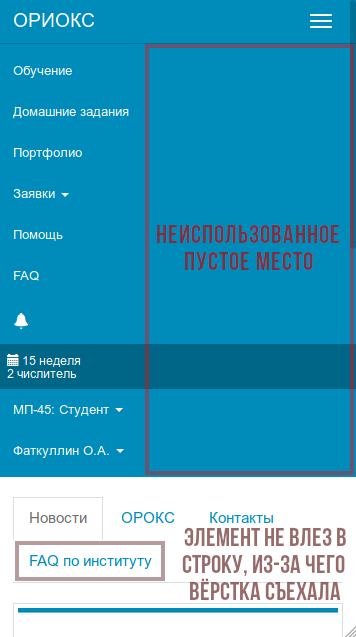
\includegraphics[width=\textwidth/2]{inc/img/orioks_mobile.png}
  \caption{Главная страница ОРИОКС с открытым меню}
  \label{fig:orioksMobile}
\end{figure}

\subsection{Сайт ОРИОКС}
\label{subsec:orioks}

\Define{Платформа}{среда выполнения, в которой должен выполняться фрагмент программного обеспечения или объектный модуль с учётом накладываемых средой ограничений и предоставляемых возможностей}
\Define{Браузер}{программное обеспечение для просмотра информации в сети Интернет}
Платформа: Браузер.

\Abbrev{БД}{база данных}
Из плюсов: cайт ОРИОКС получает информацию напрямую из БД.
Это позволяет позволяет запрашивать только ту информацию, которая нужна в данный момент для отображения страницы.
Можно, так же, отметить наличие всех перечисленных выше возможностей, за исключением просмотра расписания (но его можно посмотреть на сайте МИЭТ)~\cite{orioks}.
Графический интерфейс присутствует, но не полностью адаптирован для мобильных устройств, то есть в некоторых местах элементы интерфейса не помещаются на экране, а в других "--- наоборот слишком много неиспользованного места (см.~рис.~\ref{fig:orioksMobile}).

\Abbrev{HTML}{hypertext markup language "--- язык гипертекстовой разметки}
К минусам можно отнести отсутствие push-уведомлений, невозможность просмотра информации без интернет соединения и необходимость загружать таблицы стилей и HTML разметку для просмотра страницы.

\begin{figure}[ht]
  \centering
  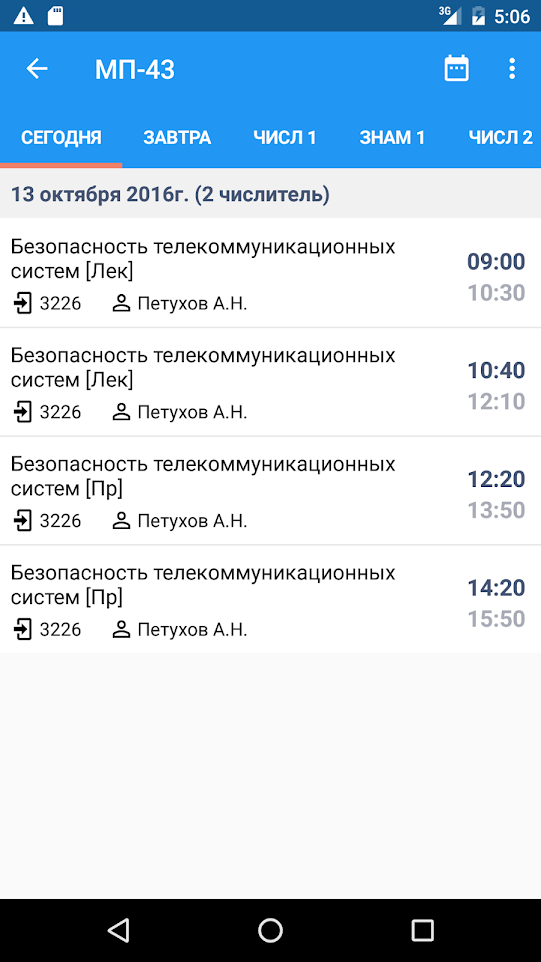
\includegraphics[width=\textwidth/2]{inc/img/miet_schedule.png}
  \caption{Экран расписания в приложении ``Расписание для МИЭТ''}
  \label{fig:mietSchedule}
\end{figure}

\subsection{Приложение ``Расписание для МИЭТ''}
\label{subsec:appMietSchedule}
Платформа: Android.
Дополнительная информация: около тысячи установок;
рейтинг на Google Play "--- 4.7 из 5;
дата последнего обновления "--- 22.04.2018.

Приложение предназначено для просмотра новостей МИЭТ и расписания любой группы с возможностью скачать его и использовать в оффлайн-режиме.
Раньше присутствовал функционал просмотра успеваемости, но из-за изменений на сайте ОРИОКС этот функционал стал недоступен~\cite{market:mietSchedule}.

Получение расписания реализовано через API, это плюс.
Для получения текущей успеваемости использовался синтаксический анализ сайта.
При таком подходе любое изменение в таблице стилей или HTML разметке сайта приводит к неработоспособности приложения, что и случилось.

Из требуемых возможностей присутствует просмотр и кэширование расписания, это позволяет просматривать его без интернет-соединения
Просмотр текущих предметов, успеваемости, списка долгов и пересдач невозможен.

Графический интерфейс присутствует, но не соответствует требованиям Material Design.
Например, слишком маленькие отступы от краёв экрана (см.~рис.~\ref{fig:mietSchedule}).

\begin{figure}[ht]
  \centering
  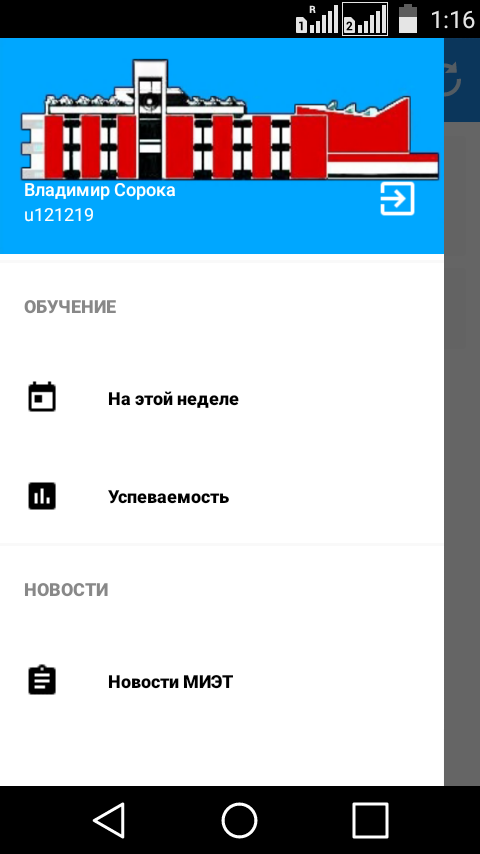
\includegraphics[width=\textwidth/2]{inc/img/orioks_live.png}
  \caption{Главный экран с открытым меню в приложении ``Ориокс Live''}
  \label{fig:orioksLive}
\end{figure}

\subsection{Приложение ``ОРИОКС Live''}
\label{subsec:appOrioksLive}
Платформа: Android.
Дополнительная информация: около тысячи установок;
рейтинг на Google Play "--- 3.9 из 5;
дата последнего обновления "--- 30.09.2015.

Приложение предназначено для просмотра успеваемости, списка контрольных мероприятий и информации о преподавателях~\cite{market:orioksLive}.

Данные получаются при помощи непубличного программного интерфейса, но интерфейс был удалён, т.к. был сделан неофициально и работа с ОРИОКС стала невозможна.
Приложение не обновлялось с 2015 года и на данный момент не работает.

Заявленный функционал проверить не удалось из-за невозможности авторизации, поэтому все эти возможности отметим как отсутствующие.
Рабочей осталась только возможность просмотра новостей.

Графический интерфейс присутствует, но не соответствует требованиям Material Design.
Неправильные отступы, слишком контрастные цвета (см.~рис.~\ref{fig:orioksLive}).

\begin{figure}[ht]
  \centering
  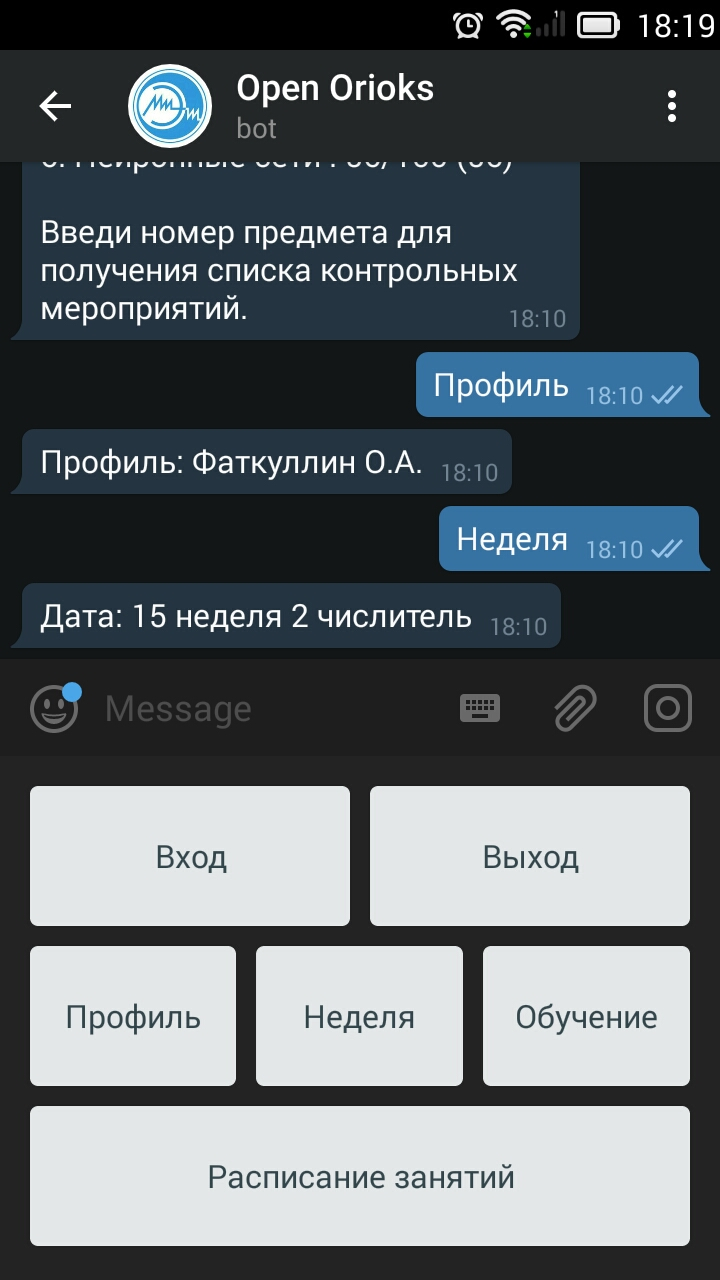
\includegraphics[width=\textwidth/2]{inc/img/open_orioks.jpg}
  \caption{Интерфейс управления Telegram-ботом ``Open Orioks''}
  \label{fig:openOrioks}
\end{figure}

\subsection{Telegram-бот ``Open Orioks''}
\label{subsec:botOpenOrioks}
Платформа: Telegram.
Дополнительная информация: последнее обновление "--- 12.10.2017.

Бот позволяет просматривать расписание на день, текущую успеваемость и список контрольных мероприятий по каждому предмету.

Для получения данных используется синтаксический анализ (как и в пункте~\ref{subsec:appMietSchedule}), но за счёт того, что данные всех студентов обновляются раз в полчаса и сохраняются в хранилище бота, скорость получения данных конечным пользователем сравнима со скоростью получения данных из БД~\cite{github:openOrioks}.

Собственного графического интерфейса нет.
Взаимодействие с ботом производится через текстовые сообщения в мессенджере Telegram.
Использование при отсутствии интернета невозможно, но можно просматривать предыдущие ответы бота, что можно считать частичным кэшированием.

По итогом обзора аналогичных решений была построена таблица~\ref{tab:analogs}.
Как видно из таблицы, нет ни одного решения, которое бы соответствовало всем необходимым параметрам, что еще раз доказывает актуальность задачи.

\begin{table}[ht]
  \caption{Сравнение аналогичных решений}
  \label{tab:analogs}
  \small
  \begin{tabularx}{\textwidth}{|>{\raggedright}m{.203\textwidth}|>{\hsize=.9\hsize}C|>{\hsize=1.2\hsize}C|C|>{\hsize=.9\hsize}C|c|}
    \hline
    Критерий & Сайт ОРИОКС~\cite{orioks} & Приложение ``Расписание для МИЭТ''~\cite{market:mietSchedule} & Приложение ``ОРИОКС Live''~\cite{market:orioksLive} & Бот ``Open Orioks''~\cite{github:openOrioks} & МП СУПС \\
    \hline
    Скорость получения информации & Средняя & Высокая & Низкая  & Средняя & Высокая \\
    \hline
    Push-уведомления              & $-$     & $-$     & $-$     & $+$     & $+$     \\
    \hline
    Расписание                    & $\pm$   & $+$     & $-$     & $\pm$   & $+$     \\
    \hline
    Текущие предметы              & $+$     & $-$     & $-$     & $+$     & $+$     \\
    \hline
    Успеваемость                  & $+$     & $-$     & $-$     & $+$     & $+$     \\
    \hline
    Долги                         & $+$     & $-$     & $-$     & $-$     & $+$     \\
    \hline
    Пересдачи                     & $+$     & $-$     & $-$     & $-$     & $+$     \\
    \hline
    Графический интерфейс         & $+$     & $-$     & $-$     & $-$     & $+$     \\
    \hline
    Оффлайн доступ                & $-$     & $+$     & $-$     & $\pm$   & $+$     \\
    \hline
  \end{tabularx}
  \caption*{
    \small
    \raggedright
    $+$ -- указанная возможность присутствует\\
    $\pm$ -- указанная возможность частично присутствует\\
    $-$ -- указанная возможность отсутствует
  }
\end{table}

В приложении ``Расписание для МИЭТ'' есть кэширование, но работает оно только для расписания, так как остальные функции недоступны.
Только Telegram-бот ``Open Orioks'' предоставляет возможность push-уведомлений, но не обладает всеми требуемыми возможностями, т.к.\ при увеличении количества выполняемых задач, бот становится неудобен в использовании.


\section{Обзор мобильных платформ}
\label{sec:platforms}
Смартфоны, в виде, похожем на нынешний, появились в 2007 году, когда Стив Джобс на выставке ``Macworld Conference \& Expo'' показал миру iPhone.
Все существующие телефоны мгновенно стали устаревшими.
Рынок смартфонов был практически пуст и было понятно, что один iPhone c iOS его не покроет.
В Google в это время только думали о выпуске своего телефона, но о смартфоне речи не шло.

\Abbrev{ОС}{операционная система}
За четыре года до этого, в 2003 году, Энди Рубин, Ник Сир, Крис Уайт и Рич Майнер решили создать операционную систему для носимых устройств, которые могли бы подстраиваться под нужды пользователя.
Они основали компанию Android Inc.\ и назвали свою операционную систему Android.
Никто тогда не оценил этот стартап и в 2005 году компания была на грани банкротства, но Энди Рубин смог убедить Google, которая занималась скупкой инновационных проектов, в том, что у Android есть будущее.
Так и оказалось.

В 2007 году Google вспоминает, что они покупали стартап, направленный на разработку операционной системы для переносных устройств.
Команда Android была только рада заняться разработкой ОС, но нужно было найти производителя смартфонов, который был бы готов выпустить на рынок устройство с совершенно новой ОС.
У Nokia уже была своя ОС "--- Symbian.
Motorola в это время была ослеплена успехом Razr и вряд ли обратила бы внимание на Android.
Оставались еще LG и HTC, но LG уже решили развивать Windows Mobile вместе с Microsoft, поэтому выбор пал на HTC\@.
HTC была рада сотрудничеству с большой компанией и могла обеспечить быстрый выпуск прототипов устройств.
В 2007--2008 году Google и HTC интенсивно работали над первым смартфоном на базе Android "--- HTC Dream.
22 октября 2008 года устройство уже поступило в продажу.

\todo{Добавить инфографику с историей развития мобильных платформ.}

В 2009 году Microsoft тоже попыталась выйти на рынок смартфонов и выпустила Windows Phone 7.
Проект оказался неудачным, своего рода ``мобильная Vista''.
Продажи устройств на Windows Mobile и Symbian упали и остались только две развивающиеся ОС "--- Android и iOS\@.
Apple не позволяла сторонним компаниям использовать iOS, поэтому все взгляды обратились  на Android.

\begin{figure}[ht]
  \centering
  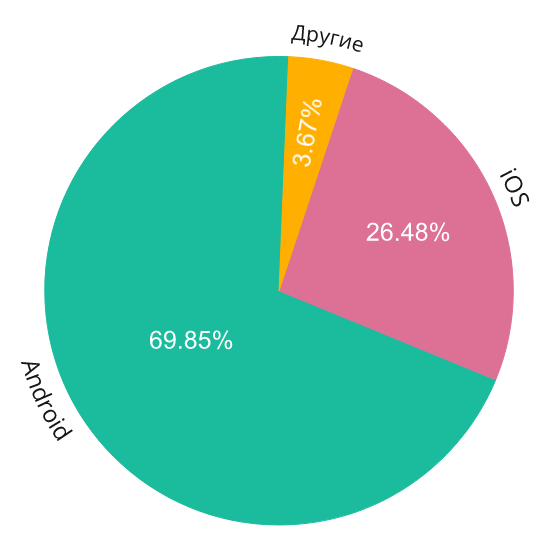
\includegraphics[width=\textwidth/2]{inc/svg/os_popularity}
  \caption{Доля устройств (данные по России)}
  \label{fig:osPopularity}
\end{figure}

Гонка Apple и Google продолжалась.
Компании улучшали свои ОС чтобы превзойти друг друга по быстродействию, безопасности, интерфейсу, функциональности, удобству использования и т.д\@.
В данный момент обе ОС достигли высокого уровня по всем направлениям, но в силу того, что Android "--- открытая система и лицензии (Apache v2 и GNU GPL v2) не запрещают устанавливать адаптировать её под любые устройства, она гораздо популярнее чем iOS\@.

Исходя из доли устройств с каждой мобильной ОС в России (см.~рис.~\ref{fig:osPopularity}), будем выбирать из двух вариантов: iOS и Android.
Разработка для iOS ведется на языке Swift или Objective-C, для работы среды разработки требуется устройство под управлением MacOS~\cite{appleDev}.
Для разработки под Android можно использовать Java или Kotlin, среда разработки не накладывает ограничений на ОС разработчика, так как доступна для Windows, Linux и MacOS~\cite{androidDev}.

\begin{table}[ht]
  \caption{Сравнение мобильных платформ}
  \label{tab:os}
  \begin{tabular*}{\textwidth}{|L|M{0.29\textwidth}|M{0.19\textwidth}|M{0.12\textwidth}|M{0.138\textwidth}|}
    \hline
    Название & Поддерживаемые языки программирования & Доля устройств (Россия)~\cite{statista:os} & Исходный код & ОС для разработки \\
    \hline
    iOS~\cite{appleDev}       & Swift, Objective-C & 26.48\% & Закрытый & MacOS \\
    \hline
    Android~\cite{androidDev} & Kotlin, Java       & 69.85\% & Открытый & GNU\textbackslash Linux, Windows, MacOS \\
    \hline
  \end{tabular*}
\end{table}

Для сравнения была составлена таблица~\ref{tab:os}.
Исходя из покрытия устройств, открытости исходного кода, ограничений на ОС для разработки и наличия опыта программирования на языках Java и Kotlin, была выбрана платформа Android.


\section{Исследование структуры ОРИОКС, концептуальная модель}
\label{sec:orioksStructure}

Функционал ОРИОКС делится на несколько частей, мы будем рассматривать только часть которая касается студентов, и говоря, например, ``инфологическая модель ОРИОКС'' будем иметь ввиду инфологическую модель студенческой части ОРИОКС\@.

На главной странице есть доступ к новостям, FAQ, портфолио, текущей успеваемости.
При открытии страницы успеваемости отображается список предметов, текущий балл по каждому из них и индикатор контрольного мероприятия (если индикатор активен, значит на этой неделе есть контрольное мероприятие по этому предмету).
Список дисциплин одинаков для всех студентов из одной группы.
Но если студент обучается по индивидуально плану, список его предметов будет отличаться.
Кроме того, у каждого студента может быть собственный список долгов, который хранится и отображается отдельно от текущих дисциплин.

Нажатие на строку предмета открывает страницу с подробной информацией, где содержится список преподавателей, форма зачёта, список ресурсов, название кафедры и список контрольных мероприятий.
Для каждого мероприятия выводится:
\begin{itemize}
  \item номер недели когда проходит мероприятие;
  \item название контрольного мероприятия;
  \item форма контроля;
  \item максимальное количество баллов;
  \item текущее количество баллов;
  \item индикатор является контрольное мероприятие обязательным или дополнительным.
\end{itemize}

Расписание не представлено в ОРИОКС, но оно есть на сайте МИЭТ.
Для каждой записи в расписании указывается:
\begin{itemize}
  \item предмет;
  \item день недели;
  \item тип недели (каждую неделю, 1/2 числитель/знаменатель);
  \item номер аудитории;
  \item номер пары;
  \item тип занятия (лабораторная работа, лекция, семинар);
  \item преподаватель.
\end{itemize}

\nocite{db}
\begin{figure}[ht]
  \centering
  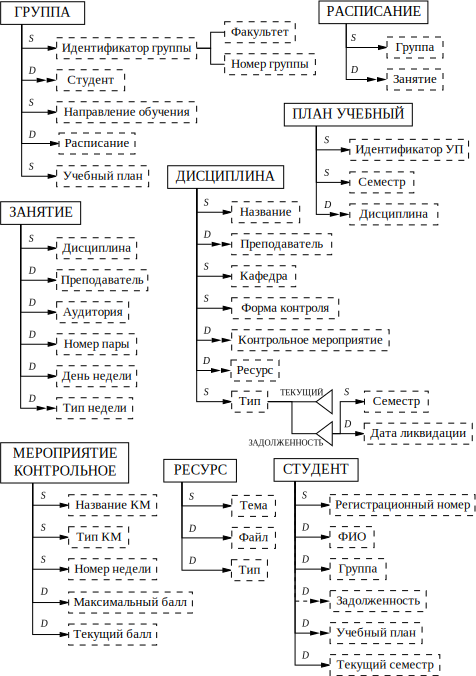
\includegraphics[width=\textwidth]{inc/svg/orioks_concept}
  \caption{Инфологическая модель ОРИОКС}
  \label{fig:orioksConcept}
\end{figure}

\begin{figure}[ht]
  \centering
  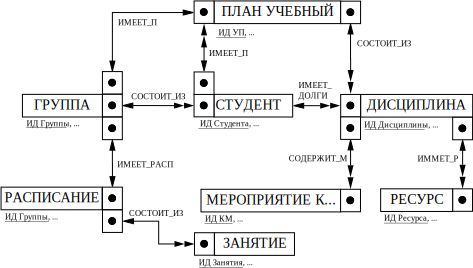
\includegraphics[width=\textwidth]{inc/svg/orioks_er}
  \caption{ER-диаграмма ОРИОКС}
  \label{fig:orioksEr}
\end{figure}

\Abbrev{ИЛМ}{инфологическая модель предметной области}
\Abbrev{ER}{entity-relationship (сущность-связь)}
Можно выделить следующие сущности: группа, студент, план на семестр, ресурс, дисциплина, контрольное мероприятие, расписание, занятие (одна запись из расписания).
Для них была построена ИЛМ (рис.~\ref{fig:orioksConcept}) и ER-диаграмма (рис.~\ref{fig:orioksEr}).


\section{Входные и выходные данные}
\label{sec:io}
В студенческой части ОРИОКС нет полей ввода, кроме формы запроса справки и формы портфолио.
Ввод осуществляется при помощи мыши и заключается в выборе элемента, о котором


\section{Постановка задачи}
\label{sec:problem}

\conclusions
\label{sec:researchConclusions}

  \chapter{Конструкторский раздел}
\label{ch:design}

\section{Выбор языка программирования}
\label{sec:language}

\section{Выбор среды разработки}
\label{sec:ide}

\section{Выбор стека технологий}
\label{sec:stack}

\section{Архитектура и алгоритм работы МП СУПС}
\label{sec:architecture}

\section{Разработка пользовательского интерфейса}
\label{sec:gui}

  \chapter{Технологический раздел}
\label{ch:tech}
В данном разделе описываются использованные технологии разработки, сборки и публикации, отладки и тестирования Android-приложений.

\section{Разработка под Android}
\label{sec:dev}
В данном подразделе рассматриваются популярные архитектурные подходы при написании приложений для Android, а так же описывается структура проекта.

\subsection{Архитектура приложения}
\label{subsec:arch}

Чаще всего Android-разработчиками используется подход под названием ``Clean Architecture'' или ``чистая архитектура''.
Изначально подход был сформулирован Бобом Мартином еще в 2012 году\cite{martin:clean} и использовался не только в Android-разработке.
Основная идея подхода состоит в том, чтобы написать приложение, которое:
\begin{itemize}
  \item не зависит от пользовательского интерфейса;
  \item не зависит от внешних ферймворков, хранилища информации и библиотек;
  \item легко тестируется.
\end{itemize}

Таким образом, в хорошо спроектированном приложении можно ``откладывать'' решения до того момента, когда их действительно необходимо принять.
Если вместо одной технологии хранения появится другая более привлекательная, или если используемая технология перестанет справляться с нагрузкой "--- возможность лёгкой смены решения сыграет на руку.
В итоге получается слоистая и гибкая архитектура, единый подход в осмыслении всего приложения~\cite{gihub:androidArch}.

\begin{figure}[ht]
  \centering
  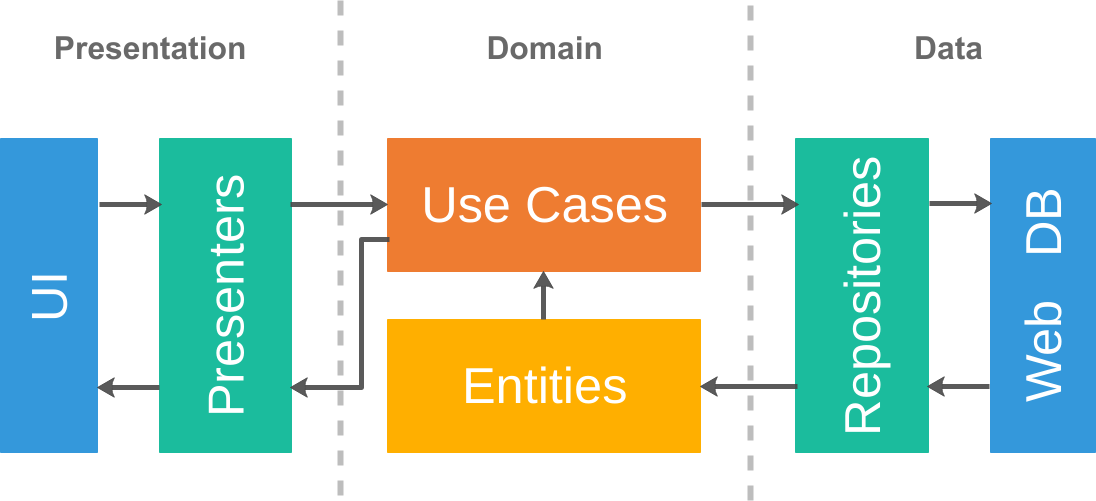
\includegraphics[width=\textwidth]{inc/img/clean_arch.png}
  \caption{Линейная диаграмма, изображающая слои чистой архитектуры}
  \label{fig:cleanArch}
\end{figure}

Изначально Роберт Мартин изобразил архитектуру как четырёхслойную ``луковицу'', у которой в центре находится слой Entity, а снаружи UI, Web, DB, но удобнее представлять чистую архитектуру в виде линейной диаграммы, изобрженной на рисунке~\ref{fig:cleanArch}.

Стрелки показывают потоки данных между слоями.
Например, событие, инициированное пользователем, идет в Presenter, тот образается к Use Case.
Use Case делает запрос в Repository, который получает данные, создает Entity и передает его в UseCase.
Так Use Case получает все нужные ему Entity.
Затем, применив их и свою логику, получает результат, который передает обратно в Presenter.
А тот, в свою очередь, отображает результат в UI~\cite{habr:clean}.

Разработку приложения удобнее вести сверху вниз, то есть сначала реализовывать внешние слои и постепенно углубляться в внутренним.
Это позволяет максимально быстро увидеть результат, кроме того, всегда удобно отталкиваться от того, что должен видеть пользователь.

Как видно из рисунка~\ref{fig:cleanArch}, проект удобно делить на три части: presentation, domain и data.
Модуль presentation зависит от Android API, так как взаимодействует с графическим интерфейсом и прочими функциями системы.
Слой data, так же, частично зависит от Android API т.к. в нём происходит взаимодействие с сетью, файлами и базами данных.
Слой domain напротив полностью независим от Android и в нём содержится вся бизнес-логика приложения.

\subsection{Структура проекта}
\label{subsec:struct}

Есть два типа разбиения структуры проекта: по слоям и по возможностям (или функциям).
При разбиении проекта по слоям возникает риск захламлённости пакетов, т.к. при использовании чистой архитектуры количество классов увеличивается довольно быстро.
Разбиение по возможностям, мало того, что лишено этого недостатка, но еще и обладает дополнительными преимуществами:
\begin{enumerate}
  \item Можно узнать о возможностях приложения только посмотрев на структуру папок;
  \item Легко добавлять новые возможности в приложение;
  \item Легко удалять возможности, для этого достаточно лишь удалить директорию;
  \item Легко ориентироваться в коде, когда он организован таким образом;
  \item Позволяет переиспользовать код в других проектах;
  \item Разработчики могут работать независимо друг от друга в разных пакетах~\cite{medium:pbf}.
\end{enumerate}

\begin{figure}[!ht]
  \minipage[b]{0.32\textwidth}
    \begin{forest}
      [\textbf{Presentation}
        [internal
          [di]
        ]
        [presentation
          [feature
            [activity]
            [fragment]
            [presenter]
            [\textit{view}]
          ]
        ]
        [utils]
      ]
    \end{forest}
    \caption{Структура модуля Presentation}\label{fig:presentationStruct}
  \endminipage\hfill
  \minipage[b]{0.32\textwidth}
    \begin{forest}
      [\textbf{Domain}
        [model]
        [\textit{repository}]
        [usecase]
        [utils]
      ]
    \end{forest}
    \caption{Структура модуля Domain}\label{fig:domainStruct}
  \endminipage\hfill
  \minipage[b]{0.32\textwidth}%
    \begin{forest}
      [\textbf{Data}
        [converter]
        [entity]
        [network]
        [repository]
        [storage]
        [utils]
      ]
    \end{forest}
    \caption{Структура модуля Data}\label{fig:dataStruct}
  \endminipage
\end{figure}

При разбивке проекта по возможностям, структура проекта имеет вид как на рисунках~\ref{fig:presentationStruct}--\ref{fig:dataStruct}.
Жирным шрифтом выделены названия модулей, а курсивом директории, которые содержат только абстракции.

\section{Сборка и публикация приложения}
\label{sec:build}
В этом подразделе описываются:
\begin{itemize}
  \item процессы сборки и публикации приложения;
  \item работа с Gradle в Android-проектах;
  \item подпись APK файла приложения;
  \item настройка сервиса непрерывной интеграции для работы с Android-проектом.
\end{itemize}

\subsection{Система автоматической сборки Gradle}
\label{subsec:gradle}

\Abbrev{APK}{Android package kit}
\Abbrev{DSL}{domain-specific language "--- язык, специфический для предметной области}
\Abbrev{XML}{extensible markup language "--- расширяемый язык разметки}
Для сборки приложения в APK файл при Android-разработке обычно используется Gradle.
Это система автоматизации сборки с открытым исходным кодом, ориентированная на гибкость и производительность.
В отличие от аналогов (Maven и Ant), сценарии сборки пишутся на Groovy или Kotlin DSL, а не на XML\@.
Это позволяет максимально снизить порог вхождения для программиста~\cite{gradle:docs}.

Gradle является официальным инструментом сборки для Android и поддерживает многие популярные языки и технологии.
Время сборки сильно уменьшается за счёт того, что при сборке используются результаты прошлых сборок, выполняется сборка только измененных файлов (инкрементальная сборка) и независимые между собой задачи выполняются параллельно.
Gradle поддерживается всеми IDE для Android-разработки, в том числе IntelliJ IDEA\@.

При создании нового проекта в IDEA можно выбрать какой DSL использовать для сценариев сборки.
В процессе разработки МП СУПС используется Kotlin DSL, т.к. язык проекта "--- Kotlin.
После указания основных настроек (название приложения, домен, целевая версия и т.д.) создаются стандартные сценарии сборки для всего проекта и для модуля 'app', в котором содержится код приложения.
Это обусловлено тем, что в проекте может быть несколько модулей, например, модули data, domain и presentation при использовании чистой архитектуры.
Gradle и Kotlin DSL обновляются чаще чем инструменты разработки Android, поэтому созданные по умолчанию сценарии сборки могут не работать в силу того, что Kotlin DSL находится в стадии активной разработки и не гарантирует обратную совместимость, а шаблоны рассчитаны на старые версии.

Помимо сценариев сборки в Gradle есть еще файлы настроек:
\begin{itemize}
  \item \code{gradle.properties} содержит настройки Gradle (здесь, например, можно выставить ограничение потребления памяти);
  \item \code{settings.gradle.kts} содержит список модулей, которые нужно подключить;
  \item \code{gradle-wrapper.properties} (находится по пути \code{gradle/wrapper/}) содержит настройки обёртки Gradle (Gradle wrapper).
\end{itemize}

Gradle позволяет дописывать собственные вспомогательные классы, которые можно будет использовать при написании сценария сборки.
Такие классы помещают в модуль \code{buildSrc}, который подключён по умолчанию и этот собирается перед сборкой остальных модулей.
Еще одна возможность организации структуры сценариев сборки "--- разбивка сценария на несколько файлов, отвечающих за разные аспекты сборки.
Например, выделить отдельный файл, в котором будет собрана вся работа с зависимостями.
В Gradle для подключения внешних файлов сценариев предусмотрена функция:
\codeline{kotlin}{project.apply { from("path/to/script.gradle.kts") }}

Все необходимые задачи, такие как настройка проекта для работы с Android, сборка приложения в APK, подпись его ключом и пр.\ выделены в отдельный плагин "--- Android Gradle Plugin.
Подключение этого плагина осуществляется в сценарии уровня проекта в секции \code{buildscript.dependencies} (листинг~\ref{lst:rootBuildKts}).

\begin{listing}[H]
  \kotlinfile{inc/src/rootBuild.gradle.kts}
  \caption{Подключение Android Gradle Plugin версии 3.0.1}
  \label{lst:rootBuildKts}
\end{listing}

После того, как плагин подключен, в сценарии уровня модуля, нужно указать настройки сборки Android приложения, а именно, целевую версию, минимальную допустимую версию, версию инструментов сборки, ID и версию приложения (листинг~\ref{lst:moduleBuildKts}).

\begin{listing}[H]
  \kotlinfile{inc/src/moduleBuild.gradle.kts}
  \caption{Настройка сборки Android-приложения}
  \label{lst:moduleBuildKts}
\end{listing}

\subsection{Управление зависимостями}
\label{subsec:libs}

Ни одно Android-приложение не обходится без зависимостей.
Проект всегда использует бибилиотеки, а так же может быть разбит на отдельные модули, которые зависят друг от друга.
Управление зависимостями "--- это метод декларирования, разрешения и использования зависимостей, требуемых проектом, в автоматическом режиме.

В Gradle есть инструменты для управления зависимостями, которые покрывают все типичные сценарии, встречающиеся в современных проектах по разработке ПО\@.

\begin{figure}[ht]
  \centering
  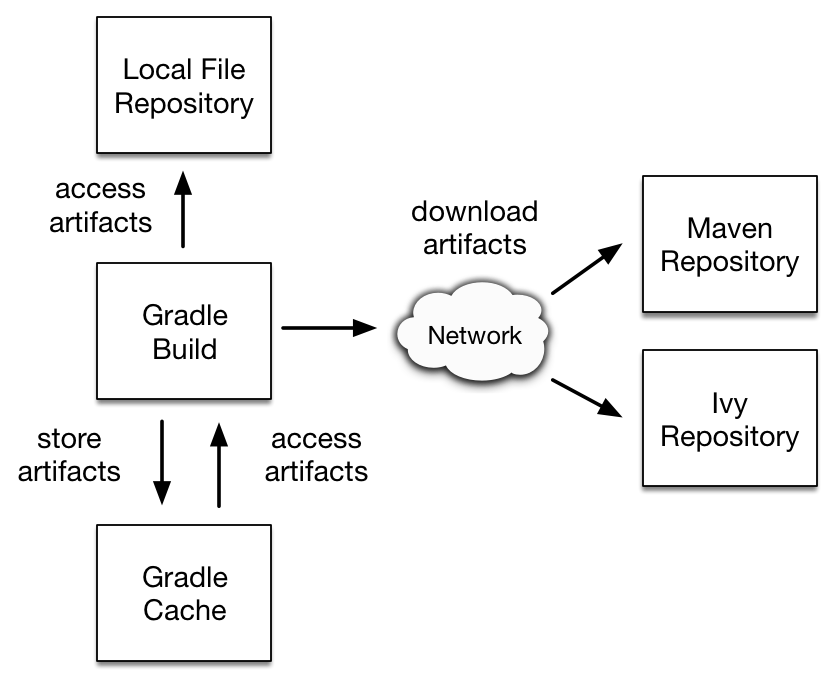
\includegraphics[width=0.7\textwidth]{inc/img/gradle_dependency_management.png}
  \caption{Управление зависимостями в Gradle}
  \label{fig:gradleDeps}
\end{figure}

Например есть проект, написанный на Java.
В некоторых файлах используются классы из Google Guava (библиотека с открытым исходным кодом, предоставляющая множество полезных функций).
Кроме того, проекту нужен JUnit для компиляции и выполнения тестов.

Guava и JUnit представляют собой зависимости этого проекта.
Программист, при написании сценария сборки, может определять зависимости для разных областей (scopes), например, для компиляции всего кода или для компиляции и выполнения тестов.
В Gradle область действия зависимости называется ``конфигурацией''.

Обычно зависимости подключаются в виде модулей.
Необходимо указать Gradle, где найти эти модули, чтобы их можно было использовать во время сборки.
Место хранения модулей называется репозиторием.
После указания репозиториев для сборки, Gradle будет знать, как находить и получать модули.
Репозитории могут быть разных типов: локальный каталог и удаленный или локальный репозиторий.
Для обеспечения совместимости с популярными хранилищами модулей Gradle может использовать Maven и Ivy репозитории

Gradle определяет требуемые зависимости во время выполнения сценария сборки.
Зависимости могут быть загружены из удаленного репозитория, извлечены из локального каталога или могут потребовать сборки другого проекта при многопроектной конфигурации.
Этот процесс называется разрешением зависимостей.

После разрешения Gradle хранит файлы зависимости в локальном кэше, называемом кэшем зависимостей.
При повторной сборке будут повторно использованы файлы, хранящиеся в кэше, чтобы избежать ненужных сетевых вызовов и ускорить сборку.

Модули могут предоставлять метаданные, то есть данные, которые дополнительно описывают модуль, например, координаты для нахождения его в репозитории, актуальную версия модуля, информацию об авторах и т.д.
В рамках метаданных модуль может объявить, что для его работы необходимы другие модули, а Gradle автоматически разрешает эти дополнительные зависимости, которые называют ``транзитивными зависимостями''.

Проекты с большим количеством зависимостей могут пострадать от антипаттерна, называемого ``ад зависимостей'' (dependency hell).
Для борьбы с этим Gradle предоставляет инструментарий для визуализации и анализа графа зависимостей проекта.

\subsubsection*{Объявление зависимостей}

Типичным примером библиотеки в Java-проекте является JUnit 4 (в Kotlin-проекте эта библиотека может быть заменена модулем \code{kotlin-test-junit}).

\begin{listing}[H]
  \kotlinfile[escapeinside=||]{inc/src/junitDependency.gradle.kts}
  \caption{Подключение JUnit 4 в качестве зависимости}
  \label{lst:junitDependency}
\end{listing}

В листинге~\ref{lst:junitDependency} приведен пример кода, который подключает JUnit в проект как зависимость для сборки и выполнения тестов.
В строке~\ref{line:repo} подключается репозиторий Maven Central, в котором находится модуль JUnit.
В строке~\ref{line:junit} происходит объявление самого JUnit, для этого указываются координаты артефакта в формате \code{<group>:<module>:<version>}.
В начале строки указана область действия зависимости или, в терминологии Gradle, конфигурация "--- \code{testImplementation}.
Существует много различных конфигураций, но самые часто используемые это \code{implementation} и \code{testImplementation}.
В первом случае зависимость используется для компиляции всего проекта, во втором только для компиляции тестового кода.

Проекты могут использовать более агрессивный подход объявления зависимостей.
Например, подключать всегда последнюю версию модуля.
Динамическая версия позволяет подключить последнюю версию или последнюю подверсию версии модуля.
Стоит помнить, что использование динамических версий несет потенциальный риск нарушения сборки.
Код перестанет компилироваться как только новая версия библиотеки не будет обратно совместима с использованной до этого.
Чтобы минимизировать риск можно динамически разрешать только минорную или патч версию и только при условии, что разработчик подключаемого модуля использует семантическое версионирование.
Gradle проверяет наличие новой версии библиотеки по прохождении 24 часов.

\begin{listing}[H]
  \kotlinfile{inc/src/junitDependencyDynamic.gradle.kts}
  \caption{Подключение JUnit 4 в качестве зависимости c динамически разрешаемой версией}
  \label{lst:junitDependencyDynamic}
\end{listing}

В сценарии, показанном в листинге~\ref{lst:junitDependencyDynamic} версия \code{4.+} будет разрешена в версию \code{4.12}, но как только появится новая минорная или патч версия, будет использоваться она.

Бывает, что разработчики публикуют ``снимки'' (snapshots) библиотеки при разработке новой версии.
В таком случае версия библиотеки не меняется, но сама библиотека обновляется.
Для разрешения такой ситуации в Gradle достаточно добавить к версии постфикс \code{-SNAPSHOT}.
По умолчанию, наличие измененной версии проверяется раз в 24 часа.

\subsection{Подпись приложения}
\label{subsec:signing}

После того как приложение собирается, нужно его подписать цифровой подписью с сертификатом, иначе его будет невозможно установить на Android-устройство.
В Android Gradle Plugin по умолчанию есть две конфигурации сборки: отладчная (debug) и релизная (release).
При отладочной сборке приложение подписывается общим отладочным ключом и доступно для профилировки.
При релизной сборке приложение должно быть подписано собственным сертификатом.

Сертификат открытого ключа, также известный как цифровой сертификат, содержит открытый ключ из пары открытого-закрытого ключей, а также некоторые другие метаданные, идентифицирующие владельца ключа (например, имя, название компании, город проживания).
Только владелец сертификата имеет соответствующий закрытый ключ.

При подписи, инструмент подписи прикрепляет к APK сертификат открытого ключа, который служит ``отпечатком пальца'', однозначно связывающим APK с владельцем, обладающим приватным ключом.
Это помогает Android гарантировать, что обновления приложения являются подлинными и исходят от оригинального автора.
Ключ, используемый для создания этого сертификата, называется ключом подписи.
Хранилище ключей "--- это бинарный файл, содержащий один или несколько закрытых ключей.

Так как ключ подписи используется для подтверждения, что обновления выпущены действительно разработчиком, сохранение его в тайне является важной задачей как для разработчика, так и для пользователей его приложений.
Можно использовать технологию Google Play App Signing для безопасного управления и хранения ключа подписи подписи приложения при помощи инфраструктуры Google или же самостоятельно хранить ключ подписи в надёжном месте.

\begin{figure}[ht]
  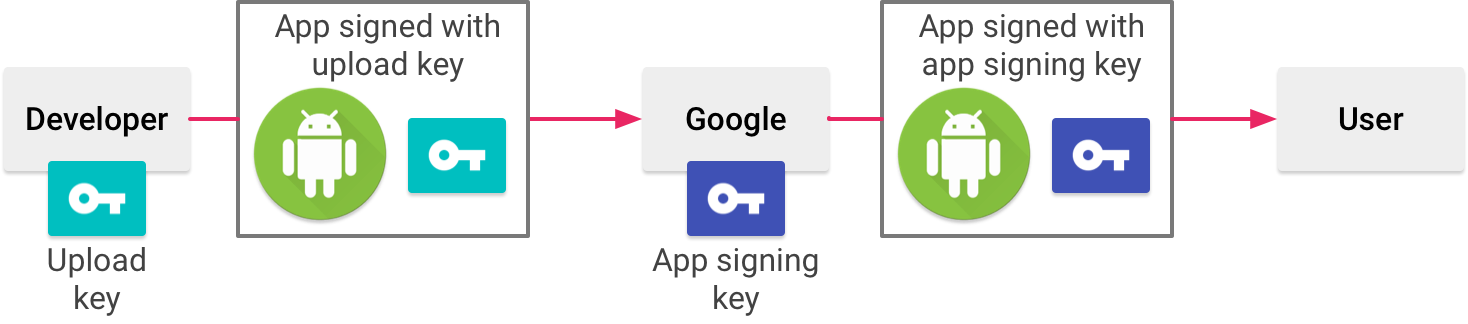
\includegraphics[width=\textwidth]{inc/img/appsigning_gpas.png}
  \caption{Подпись приложения при помощи Google Play App Signing}
  \label{fig:appsigningGpas}
\end{figure}

В случае использования Google Play App Signing, есть два ключа: ключ загрузки и ключ подписи.
Ответственность за сохранность в тайне ключа подписи лежит на Google, а ключ загрузки находится у разработчика.
Ключом загрузки разработчик подписывает приложения для загрузки в Google Play, для того чтобы подтвердить, что обновление подлинно.
Ключ подписи же загружается в Google Play один раз и приложение переподписывается им при публикации.

\begin{figure}[ht]
  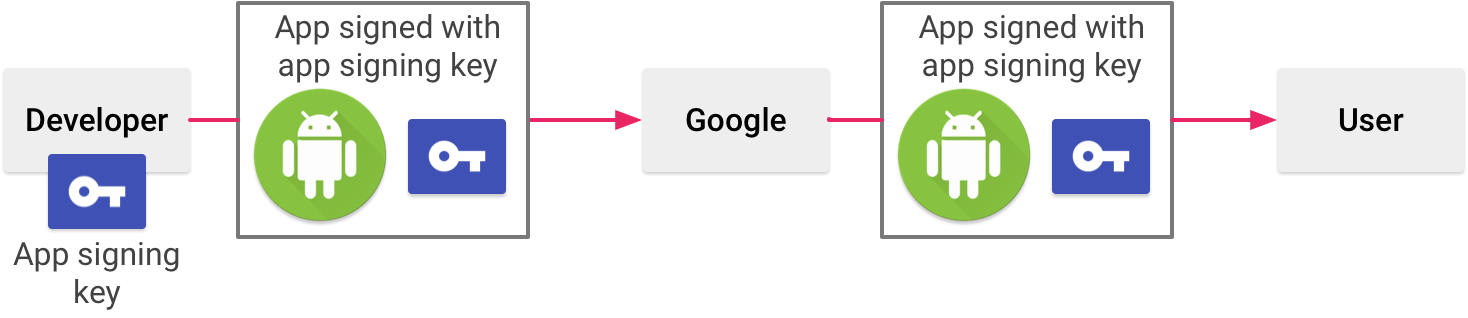
\includegraphics[width=\textwidth]{inc/img/appsigning_self.png}
  \caption{Подпись приложения при самостоятельном управлении ключом подписи}
  \label{fig:appsigningSelf}
\end{figure}

Отличие системы двухступенчатой подписи (рисунок~\ref{fig:appsigningGpas}) от одноступенчатой (рисунок~\ref{fig:appsigningSelf}) в том, что если ключ загрузки будет скомпрометирован, то его можно сменить сохранив ключ подписи.
А в силу того, что ключ подписи хранится только на серверах Google, можно не беспокоиться, что он будет скомпрометирован.

\subsubsection*{Процесс подписи APK}

Вне зависимости от того какой способ хранения ключей был выбран, необходимо создать хранилище ключей и ключ.
Для этого можно использовать встроенные в Android Studio и IntelliJ IDEA инструменты.

\begin{figure}[ht]
  \centering
  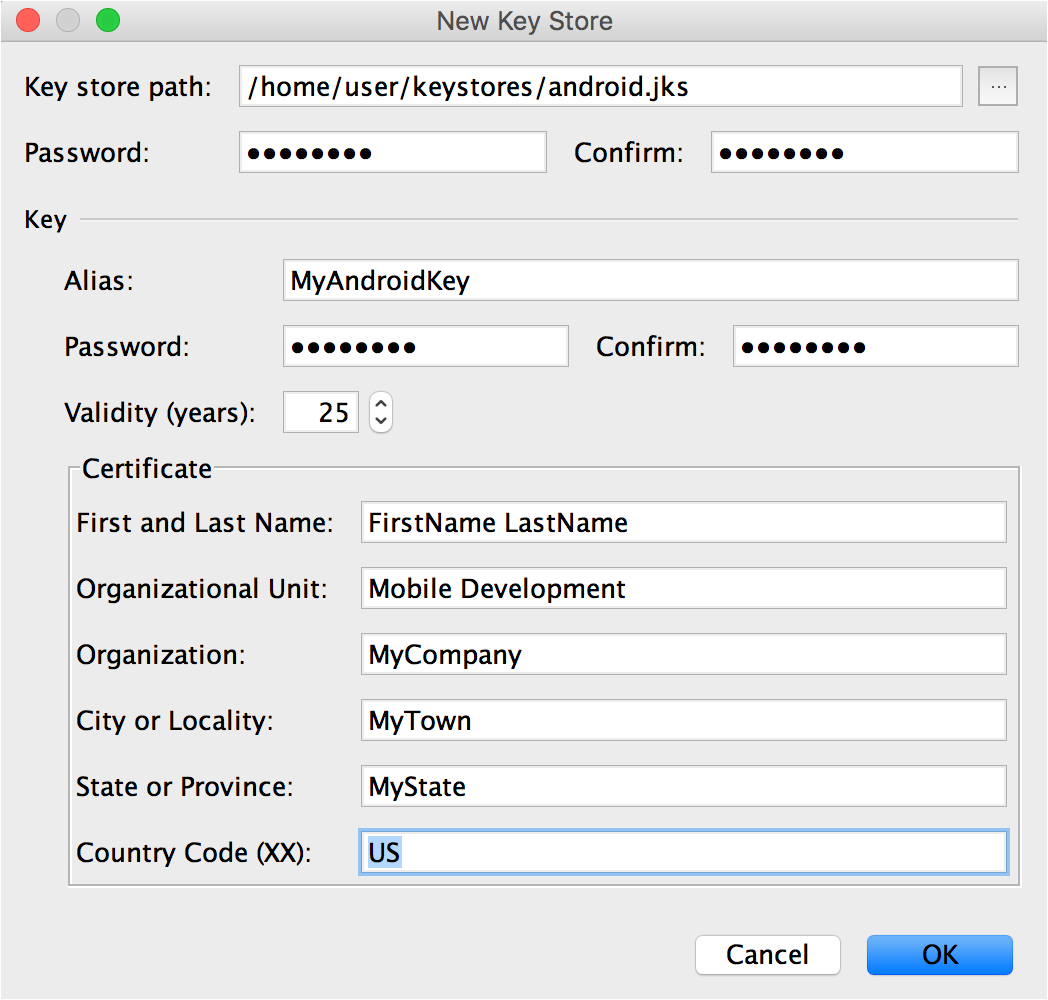
\includegraphics[width=0.7\textwidth]{inc/img/new_keystore.png}
  \caption{Создание нового ключа и хранилища ключей}
  \label{fig:newKeystore}
\end{figure}

В верхнем меню нужно выбрать \code{Build > Generate Signed APK}, после чего выбрать модуль в выпадающем меню и нажать \code{Next}.
Если нужно создать новый ключ и хранилище, нужно нажать \code{Create new}.
Откроется окно \code{New Key Store} (см.~рисунок~\ref{fig:newKeystore}), в котором нужно заполнить все поля и нажать \code{OK}.

После того как хранилище ключей и ключ созданы, нужно настроить подпись приложения в Gradle.
Для этого сначала надо добавить конфигурацию подписи, а после, ссылку на неё в релизную конфигурацию сборки как это сделано в листинге~\ref{lst:signingConfig}.

\begin{listing}[h]
  \kotlinfile{inc/src/signingConfig.gradle.kts}
  \caption{Конфигурация подписи APK в Gradle}
  \label{lst:signingConfig}
\end{listing}

Чтобы сохранить в тайне пароль от ключа и хранилища ключей при использовании VCS, можно вынести эти настройки в отдельный файл \code{.properties}, который не будет включён в систему контроля версий, и считывать их из него перед подписью.
Важно, чтобы файл хранилища ключей ни в коем случае не был включён в систему контроля версий.

\subsection{Публикация приложения}
\label{subsec:publish}

Публикация приложения "--- это основная цель разработки, т.к.\ это процесс, который делает приложение доступным для пользователей.
До, непосредственно, публикации приложение нужно подготовить.
Помимо электронной подписи, как минимум нужно удалить из приложения логирование  и отладочные атрибуты из манифеста, а так же добавить атрибуты \code{android:versionCode} и \code{android:versionName}.
Android Gradle Plugin делает это автоматически при переключении в режим релизной сборки.
Так же, необходимо тщательно протестировать приложение как минимум на одном смартфоне и одном планшете с целевой версией Android.
Если приложение зависит от внешних сервисов, то нужно убедиться, что сервисы доступны, безопасны и готовы к работе~\cite{android:publish}.

Приложение можно опубликовать несколькими способами.
Обычно для публикации используют рынки приложений, но можно, так же, опубликовать приложение на своём сайте или рассылать его непосредственно пользователям.

Публикация на рынках приложений позволяет добиться максимального охвата аудитории, но это не всегда бывает нужно, например, на стадии разработки удобнее рассылать промежуточные сборки заказчику.

Главным рынком приложений является Google Play.
Это надёжная платформа для публикации, которая позволяет продавать или распространять бесплатно Android-приложения по всему миру.
При публикации приложения на Google Play, разработчик получает набор инструментов, позволяющих анализировать продажи, тенденции на рыке, следить за ошибками во время работы приложения и т.д.
Для публикации приложения на Google Play необходим аккаунт разработчика, для регистрации которого нужно заплатить 25 USD\@.

\subsection{Непрерывная интеграция}
\label{subsec:ci}

\Abbrev{CI}{continuous integration "--- непрерывная интеграция}
Непрерывная интеграция (CI) "--- это практика разработки, когда интеграция между членами команды происходит часто и при небольших изменениях кода, а не только в конце цикла разработки.
Целью является создание более здорового программного обеспечения путем разработки и тестирования с небольшими приращениями.

В качестве платформы непрерывной интеграции выбран Travis CI, так как он поддерживает сборку Android-проектов, является открытым, бесплатным для Open Source проектов и не требует установки на собственный сервер.
Travis CI поддерживает процесс разработки, автоматически собирая и тестируя приложения, как только обнаруживает изменения кода в VCS репозитории и обеспечивает немедленную обратную связь об успехе или неудаче изменений~\cite{travis:docs}.

\begin{listing}[H]
  \yamlfile{inc/src/travisAndroid.yml}
  \caption{Файл конфигурации Travis CI для сборки Android-проекта}
  \label{lst:travisAndroid}
\end{listing}

\Abbrev{YAML}{YAML Ain't Markup Language "--- YAML -- не язык разметки}
Travis CI хранит настройки в файле \code{.travis.yml} в формате YAML\@.
Для сборки Android-приложения нужно указать настройки, аналогично тому как они указаны в листинге~\ref{lst:travisAndroid}.

Сборка может быть долгой из-за того, что Travis CI каждый раз собирает приложение ``с чистого листа''.
То есть каждый раз создаётся виртуальное окружение, в котором устанавливается JDK, подтягиваются зависимости и т.д., а значит кэширование Gradle не работает.
Чтобы ускорить сборку, можно включить кэширование, для этого нужно указать в настройке \code{cache.directories} директории, которые используются для кэша (см.~листинг~\ref{lst:travisCache}).

\begin{listing}[h]
  \yamlfile{inc/src/travisCache.yml}
  \caption{Настройки Travis CI для сохранения кэша Gradle и Android}
  \label{lst:travisCache}
\end{listing}

Удобно использовать сервисы CI для сборки и публикации промежуточных версий приложения при разработке.
Для того, чтобы настроить автоматическую публикацию приложения в GitHub Releases нужно немного изменить сценарий сборки, а именно, нужно организовать подпись приложения, при этом не скомпрометировав ключ подписи.
Для этого в Travis CI предусмотрены инструменты шифрования, которые позволяют безопасно добавлять чувствительные данные в VCS репозиторий, не боясь утечки.

Travis CI использует асимметричный алгоритм шифрования и создаёт пару RSA ключей для каждого репозитория.
Публичный ключ доступен всем, а приватный ключ Travis CI хранит в тайне, таким образом любой пользователь может зашифровать данные публичным ключом, но расшифровать их сможет только Travis CI\@.

\Abbrev{CLI}{command line interface "--- интерфейс командной строки}
Для упрощения шифрования данных есть утилита Travic CLI\@.
Чтобы зашифровать файл достаточно авторизоваться и написать одну команду:
\codeline{sh}{$ travis encrypt-file <имя_файла> --add}
После чего файл будет зашифрован и настройки для его расшифровки будут автоматически добавлены в файл конфигурации \code{.travis.yml}.

Может понадобиться зашифровать не только файл, но и строковое значение, которое нужно указать в конфиге, например токен доступа к API GitHub для публикации релиза.
Для такого случая вместо команды \code{encrypt-file} нужно использовать команду \code{encrypt}, например:
\codeline{sh}{$ travis encrypt "токен_доступа"}
Полученное значение можно использовать в настройках, оно будет автоматически расшифровано.

\begin{figure}[ht]
  \centering
  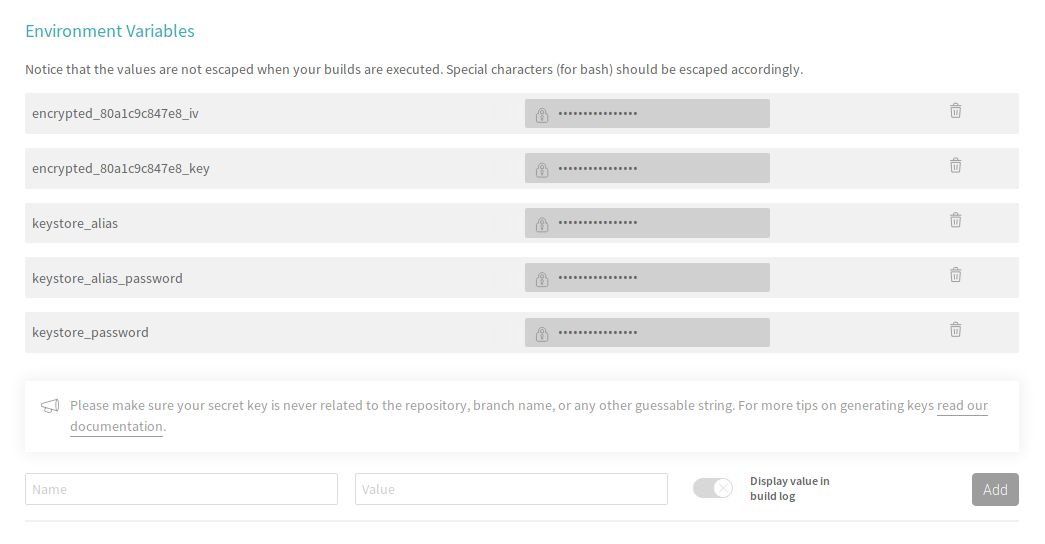
\includegraphics[width=\textwidth]{inc/img/travis_env.png}
  \caption{Веб-интерфейс Travis CI для добавления переменных окружения}
  \label{fig:travisEnv}
\end{figure}

Другой способ безопасного добавления строковых констант "--- добавление их через веб-интерфейс Travis CI (см.~рисунок~\ref{fig:travisEnv}), где достаточно написать название переменной окружения, её значение и отключить отображение переменной в логах.
Этот способ проще, чем шифровка значений при помощи утилиты.

Для подписи приложения, нужно алиас ключа, пароль от ключа и пароль от хранилища ключей поместить в переменные окружения, а сам файл хранилища ключей зашифровать и добавить в систему контроля версий.
После того как эти действия выполнены, надо изменить конфигурацию подписи, чтобы при сборке из Travis CI конфигурации подписи брались из переменных окружения.
Результат можно увидеть в листинге~\ref{lst:ciSigning}.

\begin{listing}[h]
  \kotlinfile{inc/src/ciSigning.gradle.kts}
  \caption{Конфигурация подписи приложения}
  \label{lst:ciSigning}
\end{listing}

После того как приложение успешно подписывается, можно настроить автоматическую публикацию его в GitHub Releases.
Для этого в Travis CI есть секции \code{deploy} и \code{before\_deploy}.
Пример настроек с пояснениями приведен в листинге~\ref{lst:travisDeploy}

\begin{listing}[h]
  \yamlfile{inc/src/travisDeploy.yml}
  \caption{Настройки автоматической публикации приложения из Travis CI}
  \label{lst:travisDeploy}
\end{listing}

\section{Тестирование и отладка в Android разработке}
\label{sec:testing}

В данном подразделе рассматривается тестирование и отладка Android-приложений.

\subsection{Методы тестирования программного обеспечения}
\label{subsec:testing:methods}

Методы тестирования ПО классифицируют по нескольким признакам~\cite{wiki:testing}.
По объекту тестирования:
\begin{enumerate}
  \item Функциональное тестирование "--- тестирование, основанное на проверке соответствия ПО функциональным требованиям;
  \item Тестирование юзабилити "--- тестирование с целью определения понятности и простоты использования программного обеспечения;
  \item Тестирование пользовательского интерфейса "--- проверка соответствия требованиям к пользовательскому интерфейсу;
  \item Тестирование безопасности "--- проверка уязвимости ПО к различным типам атак;
  \item Тестирование локализации "--- проверка точности перевода элементов пользовательского интерфейса, правильности перевода сопроводительной документации.
  \item Тестирование совместимости "--- тестирование с целью проверить правильность работы ПО в конкретной среде (аппаратная платформа, ОС, браузер и т.д.);
  \item Тестирование производительности "--- тестирование для определения производительности программного продукта;
  \begin{enumerate}
    \item Нагрузочное тестирование "--- определение скорости выполнения операций при разной нагрузке;
    \item Стресс-тестирование "--- оценивает надёжность и устойчивость системы в условиях превышения пределов нормального функционирования;
  \end{enumerate}
  \item Тестирование установки "--- предназначено для для проверки успешности установки, настройки, а так же обновления и удаления программного обеспечения.
\end{enumerate}

По знанию внутреннего строения системы:
\begin{enumerate}
  \item Тестирование белого ящика "--- тестирование на основе анализа внутренней структуры компонента или системы;
  \item Тестирование черного ящика "--- тестирование без каких-либо знаний о внутренней структуре компонента или системы;
  \item Тестирование серого ящика "--- комбинация тестирования белого и черного ящика.
\end{enumerate}

По степени автоматизации:
\begin{enumerate}
  \item Ручное тестирование "--- тестирование, производимое тестировщиком вручную, без использования средств автоматизации;
  \item Автоматизированное тестирование "--- тестирование выполняется при помощи специализированных средств для автоматизации тестов без участия тестировщика в непосредственном тестировании;
  \item Полуавтоматизированное тестирование "--- тестирование, выполняющееся частично вручную, частично автоматически.
\end{enumerate}

По степени изолированности:
\begin{enumerate}
  \item Юнит-тестирование "--- тестирование отдельных компонентов ПО;
  \item Интеграционное тестирование "--- тестирование взаимодействия между связанными компонентами;
  \item Системное тестирование "--- процесс тестирования системы в целом.
\end{enumerate}

По времени проведения тестирования:
\begin{enumerate}
  \item Альфа-тестирование "--- тестирование ранней версии ПО небольшой группой потенциальных пользователей или независимой группой разработчиков;
  \item Бета тестирование "--- интенсивное использование почти готового продукта с целью выявления и устранения максимального числа ошибок;
  \item Регрессионное тестирование "--- тестирование уже протестированной программы после модификации для того чтобы убедиться, что изменения работают так как было задумано;
  \item Приёмочное тестирование "--- тестирование, проводимое при приёме программного обеспечения, с целью проверки соответствия программы критериям принятия;
  \item Дымовое тестирование "--- минимальный набор тестов, направленных на проверку основного функционала программы.
\end{enumerate}

По признаку позитивности сценария:
\begin{enumerate}
  \item Позитивные тесты "--- проверка правильности работы программы при входных данных, соответствующих требованиям;
  \item Негативные тесты "--- проверка, что программа работает правильно в случае неожиданных входных данных.
\end{enumerate}

\subsection{Разработка через тестирование}
\label{subsec:testing:tdd}

\Abbrev{TDD}{Test-Driven Development "--- разработка через тестирование}
Разработка через тестирование (TDD) "--- это метод разработки ПО, при котором код пишется небольшими итерациями и предварительно для него пишется тест.
Написание тестов перед написанием кода позволяет перейти от тестирования белого ящика к тестированию чёрного ящика и заставляет разработчика думать не ``как сломать что-нибудь в этой программе'', а ``как эта программа должна работать''.

При разработке через тестирования следует соблюдать три правила TDD\@.
\begin{enumerate}
  \item Новый рабочий код пишется только после того, как будет написан юнит-тест, который не проходит.
  \item Нужно писать ровно такой объём кода для юнит-теста, чтобы тест не проходил.
  \item Нужно писать ровно такой объём рабочего кода, который необходим для прохождения юнит-теста, который в данный момент не проходит.
\end{enumerate}

Эти три правила заставляют использовать коротки рабочий цикл продолжительностью примерно полминуты.
Объём кода растёт постепенно и код уже покрыт тестами примерно на 85\%.
Высокая степень покрытия кода позволяет разработчику не бояться экспериментировать, добавлять новые возможности и изменять старые и не бояться при этом, что что-то сломается.
Кроме того, разработчик уверен, что программа работает так как он задумал.

TDD поощряет хорошую архитектуру, так как для того, чтобы модуль было легко тестировать, он должен быть изолирован.
Не получится ситуации, когда код сложно тестировать из-за большого количества зависимостей и статического кода, т.к. этого кода еще просто нет и разработчик будет писать код так, чтобы он проходил, написанные тесты.

При разработке через тестирование, полученную базу тестов можно использовать как документацию.
Каждый тестовый случай "--- демонстрация использования возможностей модуля, а так как код пишется только при наличии теста для него, то такая документация есть для всех возможностей всех модулей.

Конечно, TDD "--- не панацея и не гарантирует, что разработчик получит все перечисленные выше преимущества, т.к.\ даже при таком подходе к разработке можно продолжать писать плохой код и плохие тесты.
И, конечно, TDD, как и любой другой подход, обладает недостатками~\cite{tdd}.

\begin{enumerate}
  \item Написанные тесты нужно поддерживать.
То есть при изменении логики работы модуля нужно сначала изменить тест под новую логику, и уже после этого вносить изменения в рабочий код.
  \item На первых порах TDD замедляет разработку (но в долгосрочной перспективе разработка ускоряется).
  \item Сложно начать работать по методологии TDD, особенно, если до этого есть многолетний опыт работы по-другому.
  \item Необходимость создания тестов для всех случаев сбоев утомляет разработчика, но в долгосрочной перспективе окупается.
  \item Приходится писать большое количество тестов (что одновременно является и плюсом).
\end{enumerate}

\subsection{Тестирование пользовательского интерфейса}
\label{subsec:testing:ui}

Тестирование пользовательского интерфейса позволяет убедиться, что приложение удовлетворяет функциональным требованиям и является качественным.
Один из подходов к тестированию UI "--- ручное тестирование.
Когда тестировщик самостоятельно проходит все сценарии, которые необходимо протестировать.
Однако, ручной подход трудоёмкий и подвержен ошибкам, поэтому гораздо лучше, если тестирование UI будет выполняться автоматически.

Для кода автоматизированных тестов пользовательского интерфейса в Android предусмотрен каталог \code{src/androidTest/java}.
Android Gradle Plugin собирает тестовое приложения, опираясь на тестовый код и затем запускает тестовое приложение на устройстве, аналогичном целевому.
Устройство может быть как реальным, так и виртуальным~\cite{android:uiTesting}.

В тестовом коде можно использовать UI фреймворки для эмуляции взаимодействия пользователей с приложением.
Это позволяет писать и воспроизводить тестовые сценарии для пользовательского интерфейса.
Тестирование пользовательских взаимодействий в рамках приложения позволяет гарантировать, что пользователи не столкнутся с неожиданными результатами взаимодействии с приложением.

Фреймфорк тестирования Espresso, предоставляемый командой Android, представляет из себя API для написания тестов UI и имитации взаимодействия пользователя с приложением.
Тесты Espresso могут выполняться на устройствах с версией Android 2.3.3 (API 10) или выше.
Ключевым преимуществом Espresso перед другими фреймфорками является то, что он обеспечивает автоматическую синхронизацию пользовательских действий.
То есть, фреймворк инициирует взаимодействие с интерфейсом только тогда, когда обнаруживает, что главный поток (в котором производится отрисовка интерфейса) находится в режиме ожидания.
Благодаря этой особенности нет необходимости добавлять ненадёжные решения (например, \code{Thread.sleep()}) для ожидания отображения результата~\cite{androidTesting}.

\subsection{Отладка в IntelliJ IDEA}
\label{subsec:debug}

\conclusions
\label{sec:techConclusions}


  \backmatter %% Здесь заканчивается нумерованная часть документа и начинаются ссылки и

  \Conclusion % заключение к отчёту

Результатом выпускной квалификационной работы является рабочее мобильное приложение для сопровождения учебного процесса студентов в системе ОРИОКС.

Мобильное приложение позволяет оповещать студентов с помощью их смартфонов о событиях учебного процесса, за счёт чего повышается удобство использования ОРИОКС и повышается оперативность получения оповещений студентами.
Целевая аудитория приложения "--- студенты МИЭТ, которые заинтересованы в упрощении взаимодействия с ОРИОКС и оповещении о событиях учебного процесса.

В рамках ВКР были решены следующие задачи:
\begin{itemize}
  \item проведено исследование предметной области;
  \item проведён сравнительный анализ существующих программных решений;
  \item выбрана платформа МП;
  \item выбран язык и среда программирования;
  \item разработан алгоритм МП;
  \item разработана схема данных МП;
  \item разработан пользовательский интерфейс МП;
  \item проведены отладка и тестирование МП;
  \item разработано руководство оператора МП.
\end{itemize}
 %% заключение


  %
% Список литературы при помощи BibTeX
%

% Книги без цитирования, которые будут отображаться в конце списка
\nocite{kotlinInAction, cleanCode, gofPatterns, koldayev, gitProfessional, rxJava}

\bibliographystyle{ugost2008}
\bibliography{rpz}



  \appendix % Тут идут приложения

  \chapter{Техническое задание}
\label{ch:appendix1}

\blindtext

  \chapter{Руководство оператора}
\label{ch:appendix2}

\blindtext

  \chapter{Текст программы}
\label{ch:appendix3}
\newpage
\begin{flushright}
  ПРИЛОЖЕНИЕ~\ref{ch:appendix3}
\end{flushright}
\vfill
\begin{center}
  \uppercase{Мобильное приложение сопровождения учебного процесса студентов в системе ОРОИКС\\~\\
  Текст программы}
\end{center}
\vfill
\setcounter{page}{1}
\thispagestyle{empty}
\newpage

\begingroup
  \kotlinfile{inc/src/code/main.gradle.kts}
  \captionof{listing}{Сценарий сборки корневого проекта (build.gradle.kts)}
\endgroup
~\\
\begingroup
  \kotlinfile{inc/src/code/build.gradle.kts}
  \captionof{listing}{Сценарий сборки модуля presentation (presentation/build.gradle.kts)}
\endgroup
~\\
\begingroup
  \kotlinfile{inc/src/code/dependencies.gradle.kts}
  \captionof{listing}{Файл, где производится настройка зависимостей (presentation/build.gradle.kts)}

\begingroup
  \kotlinfile{inc/src/code/AuthFragment.kt}
  \captionof{listing}{Экрана авторизации (presentation/auth/fragment/AuthFragment.kt)}
\endgroup

\begingroup
  \kotlinfile{inc/src/code/AuthPresenter.kt}
  \captionof{listing}{Представитель экрана авторизации (presentation/auth/presenter/AuthPresenter.kt)}
\endgroup
~\\
\begingroup
\kotlinfile{inc/src/code/Validator.kt}
\captionof{listing}{Утилитарный класс для валидации полей (domain/util/Validator.kt)}
\endgroup
~\\
\begingroup
  \kotlinfile{inc/src/code/AuthView.kt}
  \captionof{listing}{Абстракция View экрана авторизации (presentation/auth/view/AuthView.kt)}
\endgroup
~\\
\begingroup
  \xmlfile{inc/src/code/screen_auth.xml}
  \captionof{listing}{Макет экрана авторизации (res/layout/screen\_auth.xml)}
\endgroup
~\\
\begingroup
  \yamlfile{inc/src/code/.travis.yml}
  \captionof{listing}{Настройки Travis CI (.travis.yml)}
\endgroup
~\\
\begingroup
  \kotlinfile{inc/src/code/ComponentHolder.kt}
  \captionof{listing}{Менеджер компонентов Dagger 2\\(internal/di/holder/common/ComponentHolder.kt)}
\endgroup
~\\
\begingroup
  \kotlinfile{inc/src/code/SubComponentHolder.kt}
  \captionof{listing}{Менеджер дочерних компонентов Dagger 2\\(internal/di/holder/common/SubComponentHolder.kt)}
\endgroup
~\\
\begingroup
  \kotlinfile{inc/src/code/MainComponent.kt}
  \captionof{listing}{Пример компонента Dagger 2 (internal/di/component/MainComponent.kt)}
\endgroup
~\\
\begingroup
  \kotlinfile{inc/src/code/BaseActivity.kt}
  \captionof{listing}{Базовая реализация Activity (presentation/common/activity/BaseActivity.kt)}
\endgroup
~\\
\begingroup
  \kotlinfile{inc/src/code/BaseFragment.kt}
  \captionof{listing}{Базовая реализация Fragment (presentation/common/fragment/BaseFragment .kt)}
\endgroup


\end{document}
